\documentclass[11pt,a4paper]{article}
\usepackage[utf8]{inputenc}
\usepackage[T1]{fontenc}
\usepackage{amsfonts}
\usepackage{amssymb}
\usepackage{mdframed}
\usepackage{tikz}
\usepackage{tkz-tab}
\usepackage{wrapfig}
\usepackage{pgfplots}
\usepackage{xcolor}
\usepackage{fancyhdr}
\usepackage{lastpage}
\usepackage{tabularx}
\pgfplotsset{compat=1.17}
\usepackage{multirow}
\usepackage[fleqn]{amsmath}
\setlength{\mathindent}{0pt}

% Défini les couleurs pour les graphiques
\definecolor{dark_green}{HTML}{008000}

% Extensions
\RequirePackage{geometry} 
\geometry{tmargin=1cm,bmargin=1.9cm,lmargin=1.9cm,rmargin=1.9cm}

% Paramètres du titre
\def\classe{$1^{\text{re}}$ Spécialité mathématiques}
\def\titre{Fonctions dérivées et applications}
\def\theme{Analyse - Cours}

% Paramètres de numérotation des pages
\fancypagestyle{custom}{
  \fancyhf{}
  \renewcommand{\headrulewidth}{0pt}
  \lfoot{Analyse - Démos}
  \cfoot{Fonctions dérivées et applications}
  \rfoot{\thepage/\pageref{LastPage}}
}

% Définition d'un type de colonne centré
\newcolumntype{Y}{>{\centering\arraybackslash}X}

\usepackage{titlesec} % Pour personnaliser les titres
\usepackage{xcolor} % Pour définir des couleurs

\title{\titre}
\author{\classe \\ \theme}
\date{}

\renewcommand{\familydefault}{\sfdefault}

% Styles pour les mdframed
\mdfdefinestyle{definitionStyle}{
    leftline=true,
    rightline=false,
    topline=false,
    bottomline=false,
    linewidth=2pt,
    linecolor=black,
    innertopmargin=0pt,
    innerbottommargin=0pt,
    innerrightmargin=0pt,
    innerleftmargin=5pt,
}

\mdfdefinestyle{proprieteStyle}{
    linewidth=1pt,
    linecolor=black,
    innertopmargin=5pt,
    innerbottommargin=5pt,
    innerrightmargin=5pt,
    innerleftmargin=5pt,
}

% Supprime l'indentation des paragraphes
\setlength{\parindent}{0pt}

\begin{document}

\maketitle
\pagestyle{custom}
\thispagestyle{custom}

\section*{I. Fonctions dérivées}

\subsection*{2. Dérivées des fonctions usuelles}

\underline {Démonstration de la propriété de la fonction carrée :} \\

Soit $f:x \mapsto x^2$. \\
Soit $x\in\mathbb{R}$ \\
Calculons $f'(x)$ \\

On calcule le taux d'accroissement de $f$ en $x$ :
\begin{equation*}
    \begin{split}
        \frac{f(x+h)-f(x)}{h}&=\frac{(x+h)^2-x^2}{h}\\
        &=\frac{x^2+2xh+h^2-x^2}{h}\\
        &=\frac{2xh+h^2}{h}=\frac{h(2x+h)}{h} \\
        &=2x+h
    \end{split}
\end{equation*}

Lorsque $h$ tend vers $0$, $2x+h$ tend vers $2x$. Donc $\displaystyle{\lim_{h\to0}\frac{f(x+h)-f(x)}{h}}=2x$.

La fonction carrée est dérivable sur $\mathbb{R}$ et sa fonction dérivée est $f'(x)=2x$. ~\\

\underline {Démonstration de la propriété de la fonction carrée :} \\

Soit $f:x\mapsto \frac{1}{x}$. \\
Soit $x\in]-\infty;0[\cup]0;+\infty[$. \\
            Calculons $f'(x)$. \\

            On calcule le taux d'accroissement de $f$ en $x$ :
            \begin{equation*}
                \begin{split}
                    \frac{f(x+h)-f(x)}{h}&=\frac{\frac{1}{x+h}-\frac{1}{x}}{h}\\
                    &=\frac{\frac{1}{(x+h)x}-\frac{1}{(x+h)x}}{h} \\
                    &=\frac{\frac{x+h}{(x+h)x}-\frac{x}{(x+h)x}}{h}\\
                    &=\frac{\frac{x-x-h}{(x+h)x}}{h}\\
                    &=\frac{-h}{(x+h)x}\times\frac{1}{h}\\
                    &=\frac{-1}{(x+h)x}
                \end{split}
            \end{equation*}

            \begin{equation*}
                \begin{split}
                    \text{Lorsque $h$ tend vers $0$,}&\text{ $x+h$ tend vers $x$}\\
                    &\text{ $(x+h)x$ tend vers $x^2$}\\
                    &\text{ $\frac{-1}{(x+h)x}$ tend vers $\frac{-1}{x^2}$}
                \end{split}
            \end{equation*}

            Donc $\displaystyle{\lim_{h\to0}\frac{f(x+h)-f(x)}{h}}=\frac{-1}{x^2}$. ~\\

            La fonction inverse est dérivable sur $]-\infty;0[\cup]0;+\infty[$ et sa fonction dérivée à pour équation $f'(x)=\frac{-1}{x^2}$.

\section*{II. Opérations sur les fonctions dérivables}

\underline{Démonstration de la formule de la dérivée d'un produit :} ~\\

Soit $f(x)=uv$. Soit $x\in I$

\begin{alignat*}{2}
     & \text{Calculons } & f'(x) & = \frac{f(x+h)-f(x)}{h}                                                                     \\
     &                   &       & = \frac{u(x+h)\times v(x+h) - u(x) \times v(x)}{h}                                          \\
     &                   &       & = \frac{u(x+h)\times v(x+h)  -u(x)\times v(x+h) +u(x)\times v(x+h)   - u(x) \times v(x)}{h} \\
     &                   &       & = v(x+h)\times \frac{u(x+h)-u(x)}{h} + u(x+h)\times \frac{v(x+h)-v(x)}{h}
\end{alignat*}

On doit calculer $\displaystyle{}\lim_{h\to0}\frac{f(x+h)-f(x)}{h}$ \\

Or $\displaystyle{}\lim_{h\to0}{v(x+h)}=v(x)$ \\

Or $\displaystyle{}\lim_{h\to0}\frac{u(x+h)-u(x)}{h}=u'(x)$ \\

Or $\displaystyle{}\lim_{h\to0}{v(x)}=u(x)$ \\

Et $\displaystyle{}\lim_{h\to0}\frac{v(x+h)-v(x)}{h}=v'(x)$
\begin{alignat*}{2}
     & \text{Donc } & \lim_{h\to0}\frac{f(x+h)-f(x)}{h} & =u'(x)\times v(x) + u(x)\times v'(x) \\
     &              & f'(x)                             & =u'(x) v(x) + u(x) v'(x)
\end{alignat*}

\section*{III. Application de la dérivation}

\subsection*{2. Étude des extrema d'une fonction}

\underline{Démonstration de la condition suffisante sur l'existence d'un extremum local} ~\\

\begin{tabular}{@{}c@{\hspace{1cm}}c@{}}
    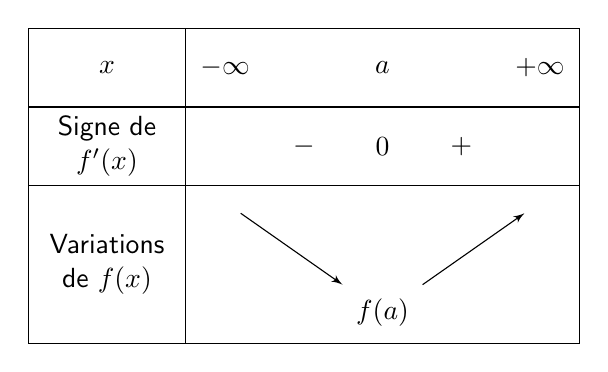
\begin{tikzpicture}
        \tkzTabInit[espcl=2]{$x$ / 1 , Signe de $f'(x)$ / 1, Variations de $f(x)$ / 2}{$-\infty$, $a$, $+\infty$}
        \tkzTabLine{,-,0,+,}
        \tkzTabVar{+/ , -/ $f(a)$, +/ }
    \end{tikzpicture} &

    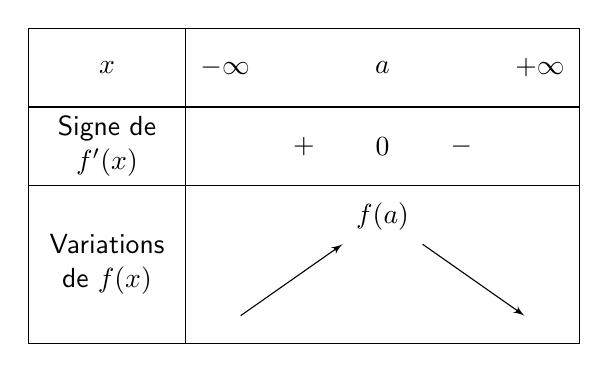
\begin{tikzpicture}
        \tkzTabInit[espcl=2]{$x$ / 1 , Signe de $f'(x)$ / 1, Variations de $f(x)$ / 2}{$-\infty$, $a$, $+\infty$}
        \tkzTabLine{,+,0,-,}
        \tkzTabVar{-/ , +/ $f(a)$, -/ }
    \end{tikzpicture}       \\

    $f(a)$ est un minimum local                                                              &
    $f(a)$ est un maximum local
\end{tabular}


\end{document}